% Created by tikzDevice version 0.12.3.1 on 2021-09-17 14:37:05
% !TEX encoding = UTF-8 Unicode
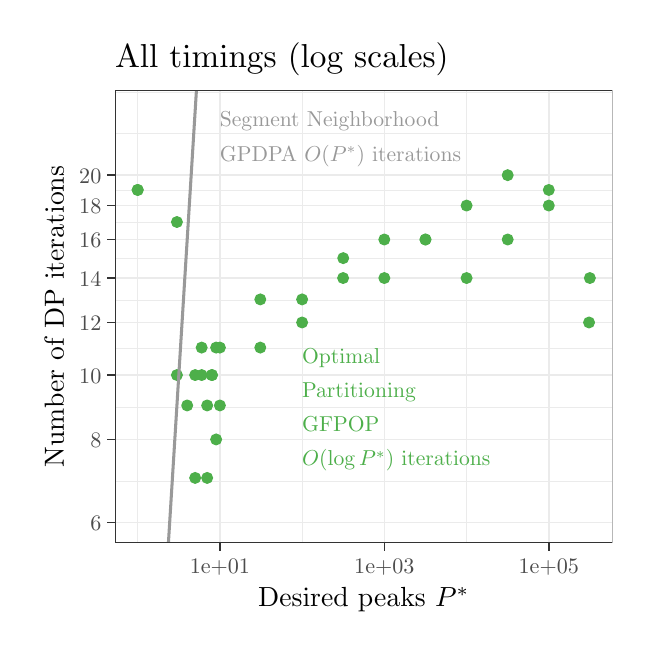
\begin{tikzpicture}[x=1pt,y=1pt]
\definecolor{fillColor}{RGB}{255,255,255}
\path[use as bounding box,fill=fillColor,fill opacity=0.00] (0,0) rectangle (216.81,216.81);
\begin{scope}
\path[clip] (  0.00,  0.00) rectangle (216.81,216.81);
\definecolor{drawColor}{RGB}{255,255,255}
\definecolor{fillColor}{RGB}{255,255,255}

\path[draw=drawColor,line width= 0.6pt,line join=round,line cap=round,fill=fillColor] (  0.00,  0.00) rectangle (216.81,216.81);
\end{scope}
\begin{scope}
\path[clip] ( 31.58, 30.61) rectangle (211.31,194.21);
\definecolor{fillColor}{RGB}{255,255,255}

\path[fill=fillColor] ( 31.58, 30.61) rectangle (211.31,194.21);
\definecolor{drawColor}{gray}{0.92}

\path[draw=drawColor,line width= 0.3pt,line join=round] ( 31.58, 53.03) --
	(211.31, 53.03);

\path[draw=drawColor,line width= 0.3pt,line join=round] ( 31.58, 79.65) --
	(211.31, 79.65);

\path[draw=drawColor,line width= 0.3pt,line join=round] ( 31.58,100.78) --
	(211.31,100.78);

\path[draw=drawColor,line width= 0.3pt,line join=round] ( 31.58,118.31) --
	(211.31,118.31);

\path[draw=drawColor,line width= 0.3pt,line join=round] ( 31.58,133.30) --
	(211.31,133.30);

\path[draw=drawColor,line width= 0.3pt,line join=round] ( 31.58,146.40) --
	(211.31,146.40);

\path[draw=drawColor,line width= 0.3pt,line join=round] ( 31.58,158.02) --
	(211.31,158.02);

\path[draw=drawColor,line width= 0.3pt,line join=round] ( 31.58,178.51) --
	(211.31,178.51);

\path[draw=drawColor,line width= 0.3pt,line join=round] ( 31.58,193.50) --
	(211.31,193.50);

\path[draw=drawColor,line width= 0.3pt,line join=round] ( 39.75, 30.61) --
	( 39.75,194.21);

\path[draw=drawColor,line width= 0.3pt,line join=round] ( 99.17, 30.61) --
	( 99.17,194.21);

\path[draw=drawColor,line width= 0.3pt,line join=round] (158.60, 30.61) --
	(158.60,194.21);

\path[draw=drawColor,line width= 0.6pt,line join=round] ( 31.58, 38.04) --
	(211.31, 38.04);

\path[draw=drawColor,line width= 0.6pt,line join=round] ( 31.58, 68.02) --
	(211.31, 68.02);

\path[draw=drawColor,line width= 0.6pt,line join=round] ( 31.58, 91.28) --
	(211.31, 91.28);

\path[draw=drawColor,line width= 0.6pt,line join=round] ( 31.58,110.28) --
	(211.31,110.28);

\path[draw=drawColor,line width= 0.6pt,line join=round] ( 31.58,126.34) --
	(211.31,126.34);

\path[draw=drawColor,line width= 0.6pt,line join=round] ( 31.58,140.26) --
	(211.31,140.26);

\path[draw=drawColor,line width= 0.6pt,line join=round] ( 31.58,152.53) --
	(211.31,152.53);

\path[draw=drawColor,line width= 0.6pt,line join=round] ( 31.58,163.51) --
	(211.31,163.51);

\path[draw=drawColor,line width= 0.6pt,line join=round] ( 69.46, 30.61) --
	( 69.46,194.21);

\path[draw=drawColor,line width= 0.6pt,line join=round] (128.88, 30.61) --
	(128.88,194.21);

\path[draw=drawColor,line width= 0.6pt,line join=round] (188.31, 30.61) --
	(188.31,194.21);
\definecolor{drawColor}{RGB}{77,175,74}
\definecolor{fillColor}{RGB}{77,175,74}

\path[draw=drawColor,line width= 0.4pt,line join=round,line cap=round,fill=fillColor] ( 39.75,158.17) circle (  1.96);

\path[draw=drawColor,line width= 0.4pt,line join=round,line cap=round,fill=fillColor] ( 53.93, 91.28) circle (  1.96);

\path[draw=drawColor,line width= 0.4pt,line join=round,line cap=round,fill=fillColor] ( 57.64, 80.30) circle (  1.96);

\path[draw=drawColor,line width= 0.4pt,line join=round,line cap=round,fill=fillColor] ( 60.52, 91.28) circle (  1.96);

\path[draw=drawColor,line width= 0.4pt,line join=round,line cap=round,fill=fillColor] ( 62.87,101.21) circle (  1.96);

\path[draw=drawColor,line width= 0.4pt,line join=round,line cap=round,fill=fillColor] ( 64.86, 54.11) circle (  1.96);

\path[draw=drawColor,line width= 0.4pt,line join=round,line cap=round,fill=fillColor] ( 66.58, 91.28) circle (  1.96);

\path[draw=drawColor,line width= 0.4pt,line join=round,line cap=round,fill=fillColor] ( 68.10,101.21) circle (  1.96);

\path[draw=drawColor,line width= 0.4pt,line join=round,line cap=round,fill=fillColor] ( 69.46, 80.30) circle (  1.96);

\path[draw=drawColor,line width= 0.4pt,line join=round,line cap=round,fill=fillColor] ( 84.06,118.62) circle (  1.96);

\path[draw=drawColor,line width= 0.4pt,line join=round,line cap=round,fill=fillColor] ( 99.17,110.28) circle (  1.96);

\path[draw=drawColor,line width= 0.4pt,line join=round,line cap=round,fill=fillColor] (114.02,133.53) circle (  1.96);

\path[draw=drawColor,line width= 0.4pt,line join=round,line cap=round,fill=fillColor] (128.87,140.26) circle (  1.96);

\path[draw=drawColor,line width= 0.4pt,line join=round,line cap=round,fill=fillColor] (143.74,140.26) circle (  1.96);

\path[draw=drawColor,line width= 0.4pt,line join=round,line cap=round,fill=fillColor] (158.60,152.53) circle (  1.96);

\path[draw=drawColor,line width= 0.4pt,line join=round,line cap=round,fill=fillColor] (173.45,163.51) circle (  1.96);

\path[draw=drawColor,line width= 0.4pt,line join=round,line cap=round,fill=fillColor] (188.31,152.53) circle (  1.96);

\path[draw=drawColor,line width= 0.4pt,line join=round,line cap=round,fill=fillColor] (203.14,126.34) circle (  1.96);

\path[draw=drawColor,line width= 0.4pt,line join=round,line cap=round,fill=fillColor] ( 39.75,158.17) circle (  1.96);

\path[draw=drawColor,line width= 0.4pt,line join=round,line cap=round,fill=fillColor] ( 53.93,146.58) circle (  1.96);

\path[draw=drawColor,line width= 0.4pt,line join=round,line cap=round,fill=fillColor] ( 60.52, 54.11) circle (  1.96);

\path[draw=drawColor,line width= 0.4pt,line join=round,line cap=round,fill=fillColor] ( 62.87, 91.28) circle (  1.96);

\path[draw=drawColor,line width= 0.4pt,line join=round,line cap=round,fill=fillColor] ( 64.86, 80.30) circle (  1.96);

\path[draw=drawColor,line width= 0.4pt,line join=round,line cap=round,fill=fillColor] ( 66.58, 91.28) circle (  1.96);

\path[draw=drawColor,line width= 0.4pt,line join=round,line cap=round,fill=fillColor] ( 68.10, 68.02) circle (  1.96);

\path[draw=drawColor,line width= 0.4pt,line join=round,line cap=round,fill=fillColor] ( 69.46,101.21) circle (  1.96);

\path[draw=drawColor,line width= 0.4pt,line join=round,line cap=round,fill=fillColor] ( 84.06,101.21) circle (  1.96);

\path[draw=drawColor,line width= 0.4pt,line join=round,line cap=round,fill=fillColor] ( 99.17,118.62) circle (  1.96);

\path[draw=drawColor,line width= 0.4pt,line join=round,line cap=round,fill=fillColor] (113.98,126.34) circle (  1.96);

\path[draw=drawColor,line width= 0.4pt,line join=round,line cap=round,fill=fillColor] (128.88,126.34) circle (  1.96);

\path[draw=drawColor,line width= 0.4pt,line join=round,line cap=round,fill=fillColor] (143.74,140.26) circle (  1.96);

\path[draw=drawColor,line width= 0.4pt,line join=round,line cap=round,fill=fillColor] (158.60,126.34) circle (  1.96);

\path[draw=drawColor,line width= 0.4pt,line join=round,line cap=round,fill=fillColor] (173.45,140.26) circle (  1.96);

\path[draw=drawColor,line width= 0.4pt,line join=round,line cap=round,fill=fillColor] (188.31,158.17) circle (  1.96);

\path[draw=drawColor,line width= 0.4pt,line join=round,line cap=round,fill=fillColor] (202.85,110.28) circle (  1.96);
\definecolor{drawColor}{gray}{0.60}

\path[draw=drawColor,line width= 1.1pt,line join=round] ( -4.73,-867.24) -- (116.07,1084.05);

\node[text=drawColor,anchor=base west,inner sep=0pt, outer sep=0pt, scale=  0.78] at ( 69.46,180.92) {Segment Neighborhood};

\node[text=drawColor,anchor=base west,inner sep=0pt, outer sep=0pt, scale=  0.78] at ( 69.46,168.63) {GPDPA $O(P^*)$ iterations};

\node[text=drawColor,anchor=base west,inner sep=0pt, outer sep=0pt, scale=  0.78] at ( 69.46,156.33) {};

\node[text=drawColor,anchor=base west,inner sep=0pt, outer sep=0pt, scale=  0.78] at ( 69.46,144.04) {};
\definecolor{drawColor}{RGB}{77,175,74}

\node[text=drawColor,anchor=base west,inner sep=0pt, outer sep=0pt, scale=  0.78] at ( 99.17, 95.36) {Optimal};

\node[text=drawColor,anchor=base west,inner sep=0pt, outer sep=0pt, scale=  0.78] at ( 99.17, 83.07) {Partitioning};

\node[text=drawColor,anchor=base west,inner sep=0pt, outer sep=0pt, scale=  0.78] at ( 99.17, 70.78) {GFPOP};

\node[text=drawColor,anchor=base west,inner sep=0pt, outer sep=0pt, scale=  0.78] at ( 99.17, 58.48) {$O(\log P^*)$ iterations};
\definecolor{drawColor}{gray}{0.20}

\path[draw=drawColor,line width= 0.6pt,line join=round,line cap=round] ( 31.58, 30.61) rectangle (211.31,194.21);
\end{scope}
\begin{scope}
\path[clip] (  0.00,  0.00) rectangle (216.81,216.81);
\definecolor{drawColor}{gray}{0.30}

\node[text=drawColor,anchor=base east,inner sep=0pt, outer sep=0pt, scale=  0.80] at ( 26.63, 35.03) {6};

\node[text=drawColor,anchor=base east,inner sep=0pt, outer sep=0pt, scale=  0.80] at ( 26.63, 65.01) {8};

\node[text=drawColor,anchor=base east,inner sep=0pt, outer sep=0pt, scale=  0.80] at ( 26.63, 88.26) {10};

\node[text=drawColor,anchor=base east,inner sep=0pt, outer sep=0pt, scale=  0.80] at ( 26.63,107.26) {12};

\node[text=drawColor,anchor=base east,inner sep=0pt, outer sep=0pt, scale=  0.80] at ( 26.63,123.33) {14};

\node[text=drawColor,anchor=base east,inner sep=0pt, outer sep=0pt, scale=  0.80] at ( 26.63,137.24) {16};

\node[text=drawColor,anchor=base east,inner sep=0pt, outer sep=0pt, scale=  0.80] at ( 26.63,149.52) {18};

\node[text=drawColor,anchor=base east,inner sep=0pt, outer sep=0pt, scale=  0.80] at ( 26.63,160.50) {20};
\end{scope}
\begin{scope}
\path[clip] (  0.00,  0.00) rectangle (216.81,216.81);
\definecolor{drawColor}{gray}{0.20}

\path[draw=drawColor,line width= 0.6pt,line join=round] ( 28.83, 38.04) --
	( 31.58, 38.04);

\path[draw=drawColor,line width= 0.6pt,line join=round] ( 28.83, 68.02) --
	( 31.58, 68.02);

\path[draw=drawColor,line width= 0.6pt,line join=round] ( 28.83, 91.28) --
	( 31.58, 91.28);

\path[draw=drawColor,line width= 0.6pt,line join=round] ( 28.83,110.28) --
	( 31.58,110.28);

\path[draw=drawColor,line width= 0.6pt,line join=round] ( 28.83,126.34) --
	( 31.58,126.34);

\path[draw=drawColor,line width= 0.6pt,line join=round] ( 28.83,140.26) --
	( 31.58,140.26);

\path[draw=drawColor,line width= 0.6pt,line join=round] ( 28.83,152.53) --
	( 31.58,152.53);

\path[draw=drawColor,line width= 0.6pt,line join=round] ( 28.83,163.51) --
	( 31.58,163.51);
\end{scope}
\begin{scope}
\path[clip] (  0.00,  0.00) rectangle (216.81,216.81);
\definecolor{drawColor}{gray}{0.20}

\path[draw=drawColor,line width= 0.6pt,line join=round] ( 69.46, 27.86) --
	( 69.46, 30.61);

\path[draw=drawColor,line width= 0.6pt,line join=round] (128.88, 27.86) --
	(128.88, 30.61);

\path[draw=drawColor,line width= 0.6pt,line join=round] (188.31, 27.86) --
	(188.31, 30.61);
\end{scope}
\begin{scope}
\path[clip] (  0.00,  0.00) rectangle (216.81,216.81);
\definecolor{drawColor}{gray}{0.30}

\node[text=drawColor,anchor=base,inner sep=0pt, outer sep=0pt, scale=  0.80] at ( 69.46, 19.62) {1e+01};

\node[text=drawColor,anchor=base,inner sep=0pt, outer sep=0pt, scale=  0.80] at (128.88, 19.62) {1e+03};

\node[text=drawColor,anchor=base,inner sep=0pt, outer sep=0pt, scale=  0.80] at (188.31, 19.62) {1e+05};
\end{scope}
\begin{scope}
\path[clip] (  0.00,  0.00) rectangle (216.81,216.81);
\definecolor{drawColor}{RGB}{0,0,0}

\node[text=drawColor,anchor=base,inner sep=0pt, outer sep=0pt, scale=  1.00] at (121.45,  7.63) {Desired peaks $P^*$};
\end{scope}
\begin{scope}
\path[clip] (  0.00,  0.00) rectangle (216.81,216.81);
\definecolor{drawColor}{RGB}{0,0,0}

\node[text=drawColor,rotate= 90.00,anchor=base,inner sep=0pt, outer sep=0pt, scale=  1.00] at ( 13.04,112.41) {Number of DP iterations};
\end{scope}
\begin{scope}
\path[clip] (  0.00,  0.00) rectangle (216.81,216.81);
\definecolor{drawColor}{RGB}{0,0,0}

\node[text=drawColor,anchor=base west,inner sep=0pt, outer sep=0pt, scale=  1.20] at ( 31.58,202.26) {All timings (log scales)};
\end{scope}
\end{tikzpicture}
